\documentclass{article}

\usepackage[utf8]{inputenc}   %for german letters ä,ö...
\usepackage[english]{babel}   %german settings
\usepackage{amsmath}
\usepackage{amssymb}
\usepackage{tikz,pgfplots}
\usetikzlibrary{patterns}
\usepackage[justification=centering]{caption}
\usepackage[left=2.5cm,right=2.5cm,top=2cm,bottom=3cm]{geometry}
\usepackage[tight-spacing=true]{siunitx}
\usepackage{booktabs}
\usepackage[outdir=./]{epstopdf}
\usepackage{subcaption}
\usepackage{placeins}
\usepackage{esdiff}

\usepackage{mathrsfs}
\usetikzlibrary{arrows,decorations.pathmorphing}
\newcommand{\degre}{\ensuremath{^\circ}}

\usetikzlibrary{patterns}
\tikzstyle{spring}=[thick,decorate,decoration={zigzag,pre length=0.3cm,post length=0.3cm,segment length=6}]

\sisetup{locale = UK}

\newcommand{\upd}[1]{^\mathrm{#1}}
\newcommand{\ind}[1]{_\mathrm{#1}}
\newcommand{\RM}[1]{\MakeUppercase{\romannumeral #1}}


\usepackage[backend=bibtex8,sorting=none]{biblatex}
\addbibresource{refs.bib}

\begin{document}
\setlength{\parindent}{0em}   %Einrücken verhindern
\title{Advanced Laboratory Course\\Experiment K225\\Positron Lifetime in Metals and Insulators}
\author{Kilian Bönisch \ \ \ \qquad s6kiboen@uni-bonn.de \qquad 2897138\\
  Friedrich Hübner \qquad s6frhueb@uni-bonn.de \qquad 2897111}
\date{05.09.18}

\maketitle
\thispagestyle{empty}

\newpage

\thispagestyle{empty}

\tableofcontents

\newpage

\section{Introduction}

The aim of this experiment is to examine the behaviour of positrons in metals, i.e.\ in indium. The $\beta^+$-decay of $^{22}$Na is used as the source for positrons which then thermalize in the indium probe. With the measurement of the finite lifetime of the positrons for different temperatures we find the temperature dependence of the vacancy formation enthalpy of indium. For the lifetime measurement a fast-slow-coincidence circuit is used. 


\section{Theoretical Background}

In this section we review the necessary theoretical background for setting up and understanding the MOT.

\subsection{Laser Cooling}
The general principle of laser cooling can be understood by considering atoms with two possible values of total angular momentum, i.e.\ $j=0$ and $j=1$. Both states are seperated by an energy gap $\Delta E$.
\begin{figure}[h]
  \centering
  \begin{tikzpicture}
    \draw (0,0)--(5,0) node[right] {$j=0$};
    \draw (0,2)--(5,2) node[right] {$j=1$};
    \draw [<->] (1,0.1)--(1,1.9);
    \draw (1.4,1) node {$\Delta E$};
  \end{tikzpicture}
  \caption{Two-state system as a model for atoms.}
  \label{fig:two_state}
\end{figure}

Aligning a laser beam with frequency $\omega$ on the atom(s), the cross section $\sigma(\omega)$ for the absorption of photons can be modelled by a Lorentzian
\begin{align*}
  \sigma(\omega) =\alpha \cdot \frac{1}{1+\beta (\omega-\omega_0)^2}
\end{align*}
with some constants $\alpha,\beta >0$ and the resonance frequency $\omega_0=\Delta E/\hbar$. For laser cooling one uses a laser with a frequency $\omega_\mathrm{L}$ smaller than the resonance frequency, i.e.\ $\omega_\mathrm{L} < \omega_0$ (see figure \ref{fig:detuning}). 
\begin{figure}[h]
  \centering
  \begin{tikzpicture}
    \draw [->] (0,0)--(0,3) node [left] {$\sigma$};
    \draw [->] (0,0)--(5,0) node [below] {$\omega$};
    \draw[domain=0:5, smooth, variable=\x, smaples=1000] plot ({\x},{3/(1+(\x-2.5)^2)});
    \draw [dotted] (2.5,3)--(2.5,0) node [below] {$\omega_0$};
    \draw [dotted] (1.7,1.83)--(1.7,0) node [below] {$\omega_\mathrm{L}$};
  \end{tikzpicture}
  \caption{Schematic graph of the cross section.}
  \label{fig:detuning}
\end{figure}

If the atom moves with the velocity $v$ towards the laser the laserfrequency gets blueshifted for the atom
\begin{align*}
  \omega_\mathrm{L}' = \omega_\mathrm{L} \left(1+\frac{v}{c}\right).
\end{align*}
This means that (if $v$ is not to high) the atom will absorb more photons since $\omega_\mathrm{L}<\omega_0$. Since the direction of photons being emitted spontaneously is random the atom does not get a netto momentum from the emission of many photons. However, the atom gains momentum against the direction of movement from the absorption of the photons. This momentum slows the atom down. In order not to get accelerated in the opposite direction after the slowing down one uses a second laser with the same frequency aligned from the opposite direction. In three dimensions one thus uses six laser beams on three orthogonal axes.

\subsection{Trapping Atoms}
In every spontaneous emmission the atom gains momentum in a random direction. This means that the atom will not be slowed down completely but performs a random walk with the average velocity being zero. During this random walk the atom will leave the focus of the laser beams and hence diffuse out of the cooling zone. To prevent the atoms from diffusing one needs a position dependent force. This can be achieved by the use of an inhomogeneous magnetic field. For the explanation of the effect we consider cooling in one dimension with an magnetic field depending on the position $x$ as
\begin{align*}
  B=B_0 \frac{x}{x_o}
\end{align*}
with some constants $B_0,x_0>0$. We assume that (compare to the normal Zeeman effect) the energy levels get shifted by 
\begin{align*}
  E_{j,m_j} \mapsto E_{j,m_j}+\mu B m_j
\end{align*}
with the constant magnetic moment $\mu$. This change breaks the degeneracy of the three $j=1$ states and splits the energy differences $\Delta E$ (and thus the resonance frequency $\omega_0$) into three different energies. The position dependence of the splitting can be used to get a position dependent force by using $\sigma^\pm$-polarized laser beams. $\sigma^+$- ($\sigma^-$-) polarized light can only be absorbed by the transition $m_j=0 \mapsto 1$ ($m_j=0 \mapsto -1$). With the setup of figure \ref{fig:trap} we get a force pushing the atoms to the point $x=0$.
\begin{figure}[h]
  \centering
  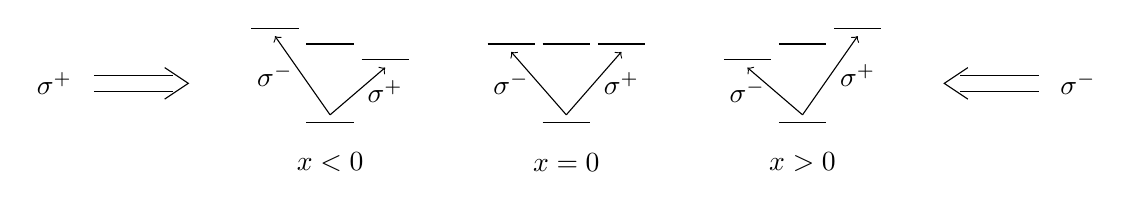
\begin{tikzpicture}
    \draw (-0.3,0)--(0.3,0);
    \draw (-0.3,1)--(0.3,1);
    \draw (-0.3-0.7,1)--(0.3-0.7,1);
    \draw (-0.3+0.7,1)--(0.3+0.7,1);
    \draw [->] (0,0.1)--(0.7,0.9); 
    \draw (0.7,0.5) node {$\sigma^+$};
    \draw [->] (0,0.1)--(-0.7,0.9); 
    \draw (-0.7,0.5) node {$\sigma^-$};
    \draw (0,-0.5) node {$x=0$}; 

    \draw (-0.3+3,0)--(0.3+3,0);
    \draw (-0.3+3,1)--(0.3+3,1);
    \draw (-0.3-0.7+3,1-0.2)--(0.3-0.7+3,1-0.2);
    \draw (-0.3+0.7+3,1+0.2)--(0.3+0.7+3,1+0.2);
    \draw [->] (0+3,0.1)--(0.7+3,0.9+0.2); 
    \draw (0.7+3,0.5+0.1) node {$\sigma^+$};
    \draw [->] (0+3,0.1)--(-0.7+3,0.9-0.2); 
    \draw (-0.7+3,0.5-0.1) node {$\sigma^-$};
    \draw (0+3,-0.5) node {$x>0$}; 

    \draw (-0.3-3,0)--(0.3-3,0);
    \draw (-0.3-3,1)--(0.3-3,1);
    \draw (-0.3-0.7-3,1+0.2)--(0.3-0.7-3,1+0.2);
    \draw (-0.3+0.7-3,1-0.2)--(0.3+0.7-3,1-0.2);
    \draw [->] (0-3,0.1)--(0.7-3,0.9-0.2); 
    \draw (0.7-3,0.5-0.1) node {$\sigma^+$};
    \draw [->] (0-3,0.1)--(-0.7-3,0.9+0.2); 
    \draw (-0.7-3,0.5+0.1) node {$\sigma^-$};
    \draw (0-3,-0.5) node {$x<0$}; 

    \draw (-6,0.6)--(-5,0.6);
    \draw (6,0.6)--(5,0.6);
    \draw (-6,0.4)--(-5,0.4);
    \draw (6,0.4)--(5,0.4);
    \draw (-5.1,0.7)--(-4.8,0.5)--(-5.1,0.3);
    \draw (5.1,0.7)--(4.8,0.5)--(5.1,0.3);
    \draw (-6.5,0.5) node {$\sigma^+$};
    \draw (6.5,0.5) node {$\sigma^-$};
  \end{tikzpicture}
  \caption{Position dependent force induced by inhomogeneous magnetic field and polarized beams. The three upper levels correspond to $m_j=-1,0,1$.}
  \label{fig:trap}
\end{figure}

In three dimensions the same effect is achieved by using an quadrupole field generated by an anti-Helmholtz configuration of coils.

\subsection{Trapping Rubidium Atoms}
The atoms that we want to cool down in this experiments are $^{85}$Rb atoms. The level structure can be found in figure \ref{fig:level_structure}. \newpage
\begin{figure}[h]
  \centering
  \includegraphics[width=0.5\textwidth]{figures/level_structure.png}
  \caption{Level structure of $^{85}$Rb.}
  \label{fig:level_structure}
\end{figure}

For the cooling we use the transition $F=3 \mapsto F'=4$. Due to rare excitations from $F=3$ to $F'=2,3$ the atoms can decay into the state $F=2$ and are then no longer available for the cooling. To get these atoms back into the cooling scheme one uses a pump laser which pumps atoms from $F=2$ to $F'=3$. 

\subsection{Polarization Spectroscopy}
For the MOT to work we need two lasers (the cooling laser and the pump laser) at two constant frequencies. In this experiment diode lasers are used. The laser diode emitts laser light of different frequencies. To filter out one frequency one uses a grating with an adjustable angle. For different angles, different frequencies are filtered out. Due to fluctuations of the temperature and the electron density the filtered out frequency is not stable. To adjust this one uses a Piezo element which adjusts the angle of the grating if the frequency changes. The error signal for the Piezo is obtained by the use of polarization spectroscopy. For the explanation of this technique we start describing the saturation spectroscopy.\\

For saturation spectroscopy the laser beam is divided into two beams. One high intensity pump beam and one low intensity test beam. Both beams are aligned on a probe ($^{85}$Rb in our case) from approximately opposite directions. The transmission of the test beam is measured with a photo diode. If the lasers are in resonance with a transition of the atoms, the pump beam will pump the atoms in the excited state. The atoms can then no longer absorb the photons of the test beam which results in a higher transmission, the so called Lamb dip (figure \ref{fig:lamb_dip}). As this mostly concerns atoms which do not move in the direction of the beams, this procedure is also called Doppler-free spectroscopy.
\begin{figure}[h]
  \centering
  \includegraphics[width=0.4\textwidth]{figures/lamb_dip.png}
  \caption{Lamb dip from saturation spectroscopy.}
  \label{fig:lamb_dip}
\end{figure}

For the polarisation spectroscopy one uses the same setup as in the saturation spectroscopy with the difference, that the pump beam is either $\sigma^+$- or $\sigma^-$-polarized. This results in an anisotropic population of the different $m_F$ states which makes the probe birefringent. As a result a linear polarized test beam then gets split into two components. One measures both transmission signals and subtracts them. The final signal has the form of the derivative of the transmission signal in figure \ref{fig:lamb_dip}. This signal can be used to lock the laser, i.e.\ it is used as the error signal for the Piezo.


\section{Procedure}

The setup of the two lasers, including the setup for the polarization spectroscopy, is already adjusted and can be seen in figure \ref{fig:setup_laser}.

\begin{figure}[h]
  \centering
  \includegraphics[width=0.5\textwidth]{figures/setup_laser.png}
  \caption{Setup of the pump laser and the cooling laser.}
  \label{fig:setup_laser}
\end{figure}

With an optical fibre the two beams get to the actual setup of the MOT which can be seen in figure \ref{fig:setup_mot}.

\begin{figure}[h]
  \centering
  \includegraphics[width=0.5\textwidth]{figures/setup_mot.png}
  \caption{Alignment of the lasers in the MOT.}
  \label{fig:setup_mot}
\end{figure}

\subsection{Adjustment of the Beams}
As a first step we adjust the alignment of the beams in figure \ref{fig:setup_mot}. It is important that the beams cross each other in the center of the quadrupole field. This can be checked with the camera es the tutor showed us where the beams should cross each other on the display. With a CCD-camera\footnote{With the camera we can see the fluorescence of the rubidium atoms in the chamber.} we make sure that the beams really cross in one point. Using an aperture we make sure that each reflected beam is parallel to the original beam. A picture of the resulting setup can be seen in figure ???.\\ \\

???\\ \\

Additionally one must make sure that the power of the laser is split into three equal parts (for each axis). To do so we measure the power of each of the three beams with the powermeter. Adjusting the $\lambda/2$-plates we get an equal intensity of about \SI{1.2}{\milli\watt} per axis (in the original laser setup). This adjustment is done with the pumping laser turned of as we are only interested in the intensity of the cooling laser beeing equal for each axis. 


\section{Evaluation}

Unfortunately we weren't able to get a MOT which lasted longer than a few seconds. This was due to the error signal for locking the cooling laser. The error signal had a frequency bias such that the desired frequency lied outside the linear part. Therefore there was no efficient feedback and the laser could easily jump to another frequency and we were effectively working with a non locked laser. We wanted to adjust the error signal, but this was denied by the tutor.

So in all following measurements we weren't able to do a full series of measurements with one MOT but rather created a new MOT every time. Errors will be calculated by Gaussian error propagation.

\subsection{Measured data}

Lense diameter: $\si{(38 \pm 3)\, \milli\meter}$

Distance between lense and MOT: $\si{(260 \pm 10)\,\milli\meter}$

Cooling beam power: $\si{(1.2 \pm 0.1)\,mW}$ per axis

Total beam power: $\si{(3.15 \pm 0.01)\,mW}$ per axis

\subsection{Beam size}

\begin{figure}
\centering
\includegraphics[width=0.7\textwidth]{data/beam.png}
\caption{Beam power over razor blade position and fit}
\label{fig:beam}
\end{figure}

The beam power is plotted over the position $a$ of the razor blade in figure \ref{fig:beam}. Since we assume a Gaussian beam the power is given by the error function, precisely $P(a) = A\qty(1-\erf(\frac{a-B}{\sqrt{2}\sigma}))$. Fitting this function to the data results in $A = \si{(1.574 \pm 0.002) mW}, B = \si{(6.12 \pm 0.09) mm}, \sigma = \si{(1.45 \pm 0.06) mm}$. The $1/e^2$ radius is then given by $4 \sigma = \si{(5.8 \pm 0.2) mm}$.

\subsection{Size of MOT}
In figure \ref{fig:mot} the MOT has dimensions $58\si{px} \times 23\si{px}$. 

\begin{figure}
\centering
\includegraphics[width=0.7\textwidth]{figures/P102018/mot_2.png}
\caption{Picture of the MOT}
\label{fig:mot}
\end{figure}

Figure \ref{fig:karton} was taken with the same camera settings. The "Bayer Makrolon" measures $\si{(21.5 \pm 0.5) \milli\meter}$ in reality and $575 \si{px}$on the foto.

\begin{figure}
\centering
\includegraphics[width=0.7\textwidth]{figures/P102018/karton.png}
\caption{Picture of some text}
\label{fig:karton}
\end{figure}

Using this gauge one can compute the dimensions of the MOT: $\si{(2.2 \pm 0.5) \milli\meter \times (0.86 \pm 0.02) \milli\meter}$. Unfortunately we don't have information about the size of the MOT in z-direction.

\subsection{Influence of the quarter waveplate}

\begin{figure}
\centering
\includegraphics[width=0.7\textwidth]{data/l42.png}
\caption{Influence of the first quarter waveplate}
\label{fig:l42}
\end{figure}

\begin{figure}
\centering
\includegraphics[width=0.7\textwidth]{data/l41.png}
\caption{Influence of the second quarter waveplate}
\label{fig:l41}
\end{figure}

In figures \ref{fig:l42} and \ref{fig:l41} the influence of the quarter waveplates on the power is given. The first waveplate (incoming beam) shows a clear drop of the power as the angle increases. As one rotates the quarter waveplate the outcoming light becomes more and more elliptical polarised. Since only the circular polarised part creates a force on the atoms this force becomes weaker and therefore less atoms will be stored in the trap. So the intensity goes down.

The second waveplate (reflected beam) shows no sensible dependence on the angle. In theory there should not be any difference, since circular polarised light has no preferred angle and therefore all angles will yield the same result. However note that we had to create a new MOT for every measurement. We think that this the causes the variation of the power for different angles.

\subsection{Loading behaviour}
Unfortunately we weren't able to observe the loading behaviour. The tutor told us we should rather measure the detuning of the laser frequency. The pump controller had a current of $0.4 \si{\milli\ampere}$ which corresponds to approximately $0.14 \cdot 10^{-3} \si{\pascal}$.

\subsection{Detuning of the laser frequency}

\begin{figure}
\centering
\includegraphics[width=0.7\textwidth]{data/oszi.png}
\caption{Observed power and according frequency spectrum (y-axis in arbitrary units)}
\label{fig:oszi}
\end{figure}

In figure \ref{fig:oszi} the observed power as function of the frequency (in bins) is given.

The position of the maximum of power is at $(8.2 \pm 0.1) \mathrm{bin}$. The leftmost peak is at $(6.9 \pm 0.1) \mathrm{bin}$ and the rightmost at $(8.6 \pm 0.1) \mathrm{bin}$. The difference between the two peaks is then $(0.7 \pm 0.1) \mathrm{bin}$ which equals (according to our lab instructions \cite{material_tutor}) $92 \si{\mega \hertz}$. Using this one can calculate the detuning to $(0.4 \pm 0.1) \mathrm{bin} = (37 \pm 9)\si{\mega \hertz}$. 



\newpage

\section{Conclusions}

We were able to create a MOT. Unfortunately it was not very stable because the locking of the laser didn't work properly. Using this we were able measure several dependencies of the florescence, e.g. from the quarter waveplates or the magnetic field and we discussed these dependencies. However since our MOT was not stable we needed to redo our MOT every time. Redoing the MOT under equal conditions yields to wide range of values for the florescence.

\FloatBarrier

\newpage

\printbibliography

\newpage

\section{Appendix}

\subsection{Gauge curves}
\begin{figure}
\centering
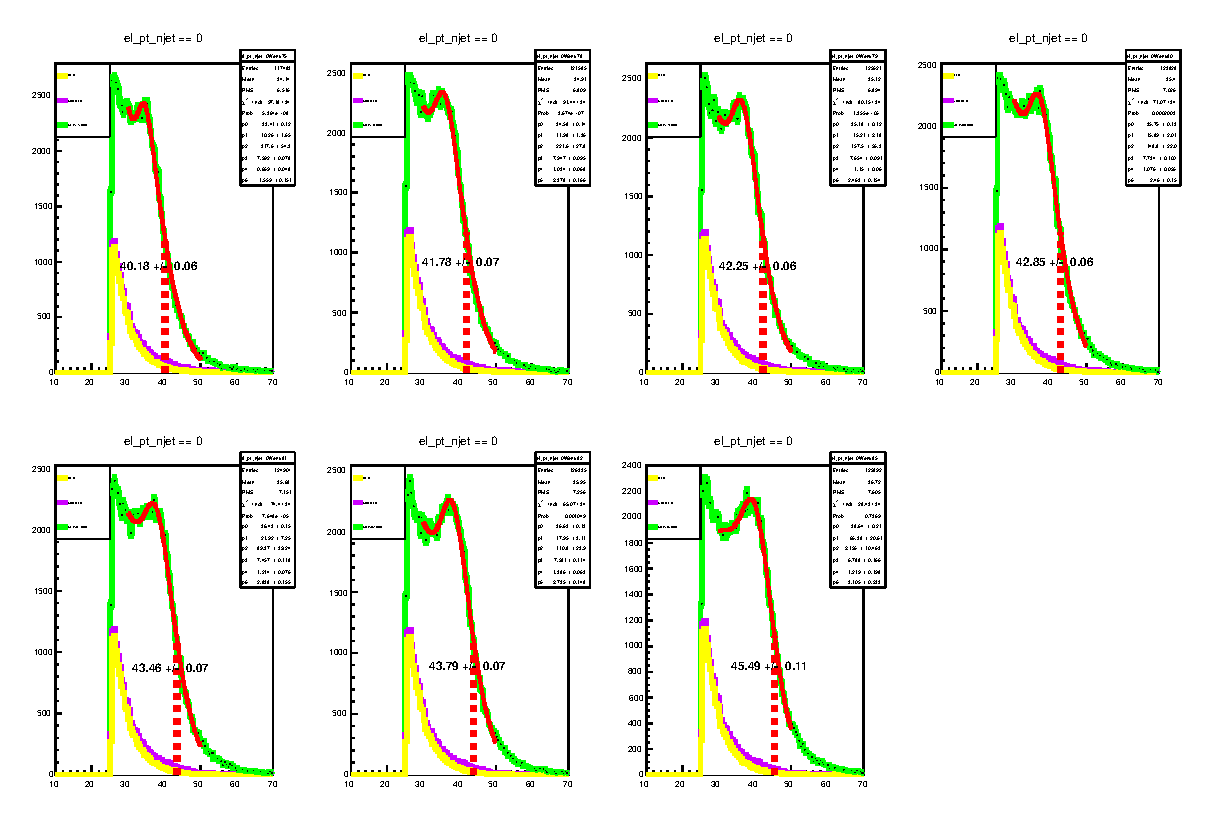
\includegraphics[width=\textwidth]{data/img/gauge_031.eps}
\caption{Gauge measurements for QCD scale factor 0.31 and fit range 30 - 50 GeV}
\end{figure}
\begin{figure}
\centering
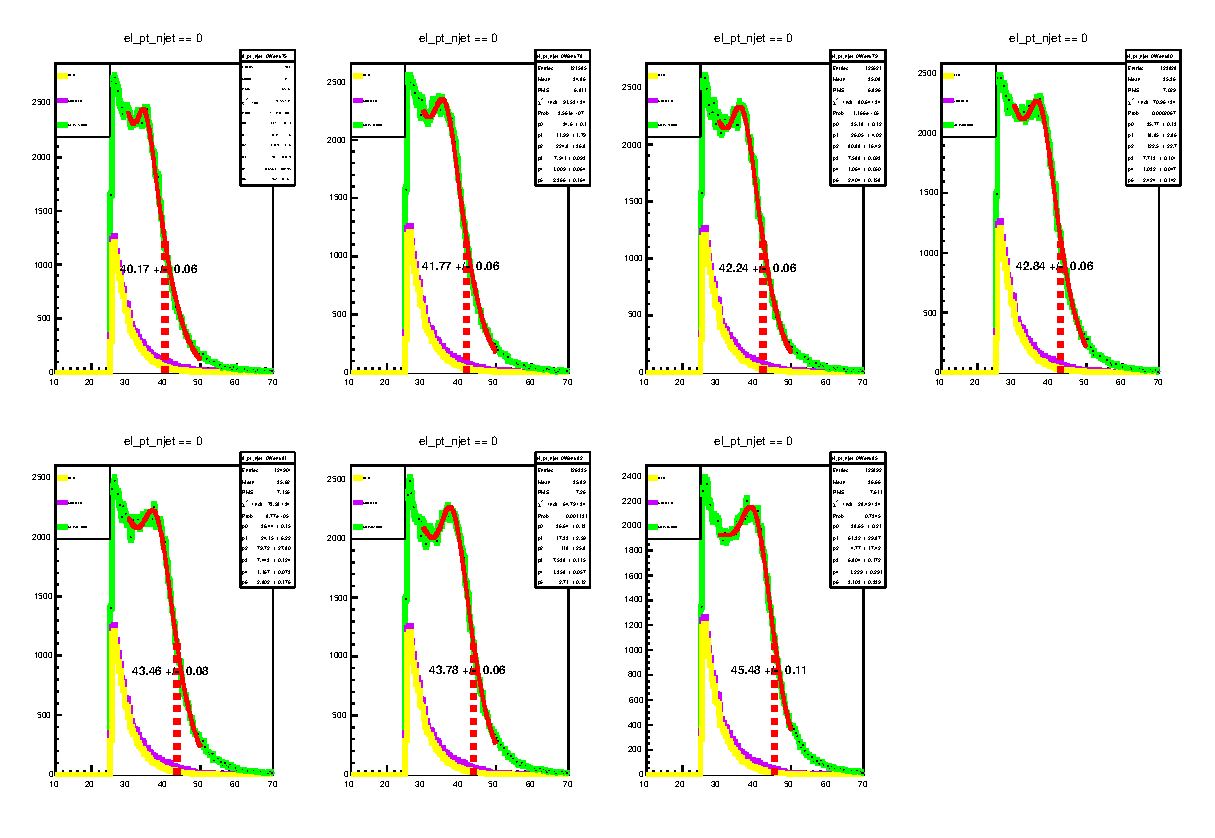
\includegraphics[width=\textwidth]{data/img/gauge_033.eps}
\caption{Gauge measurements for QCD scale factor 0.33 and fit range 30 - 50 GeV}
\end{figure}
\begin{figure}
\centering
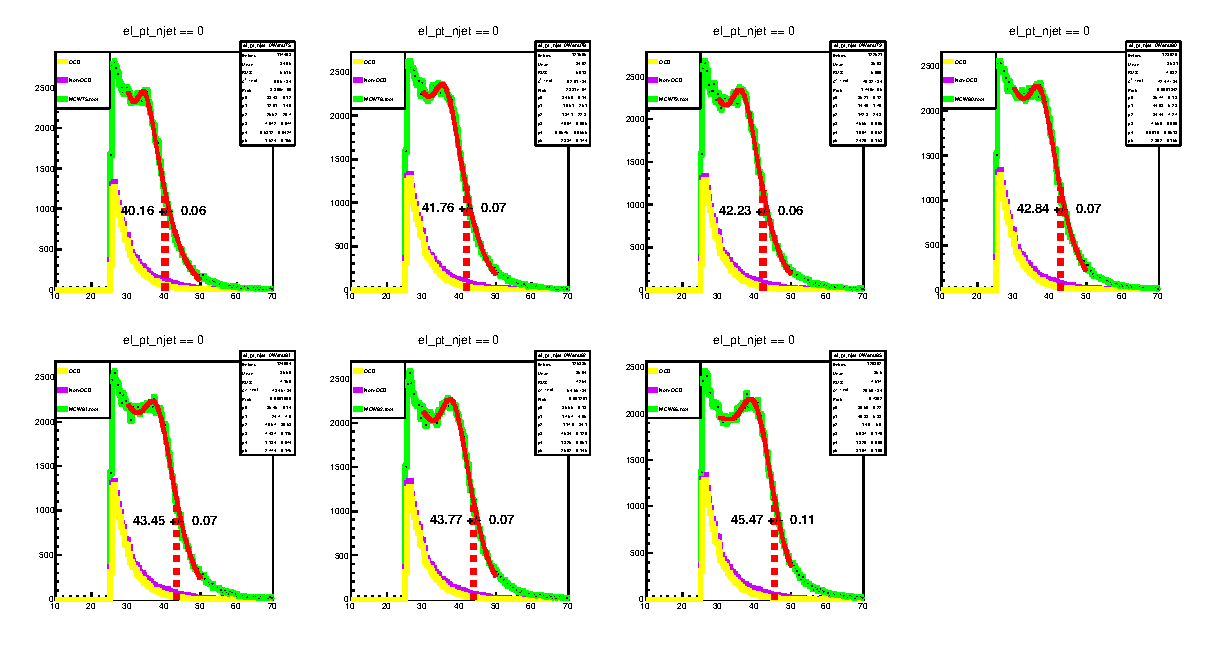
\includegraphics[width=\textwidth]{data/img/gauge_035.eps}
\caption{Gauge measurements for QCD scale factor 0.35 and fit range 30 - 50 GeV}
\end{figure}
\begin{figure}
\centering
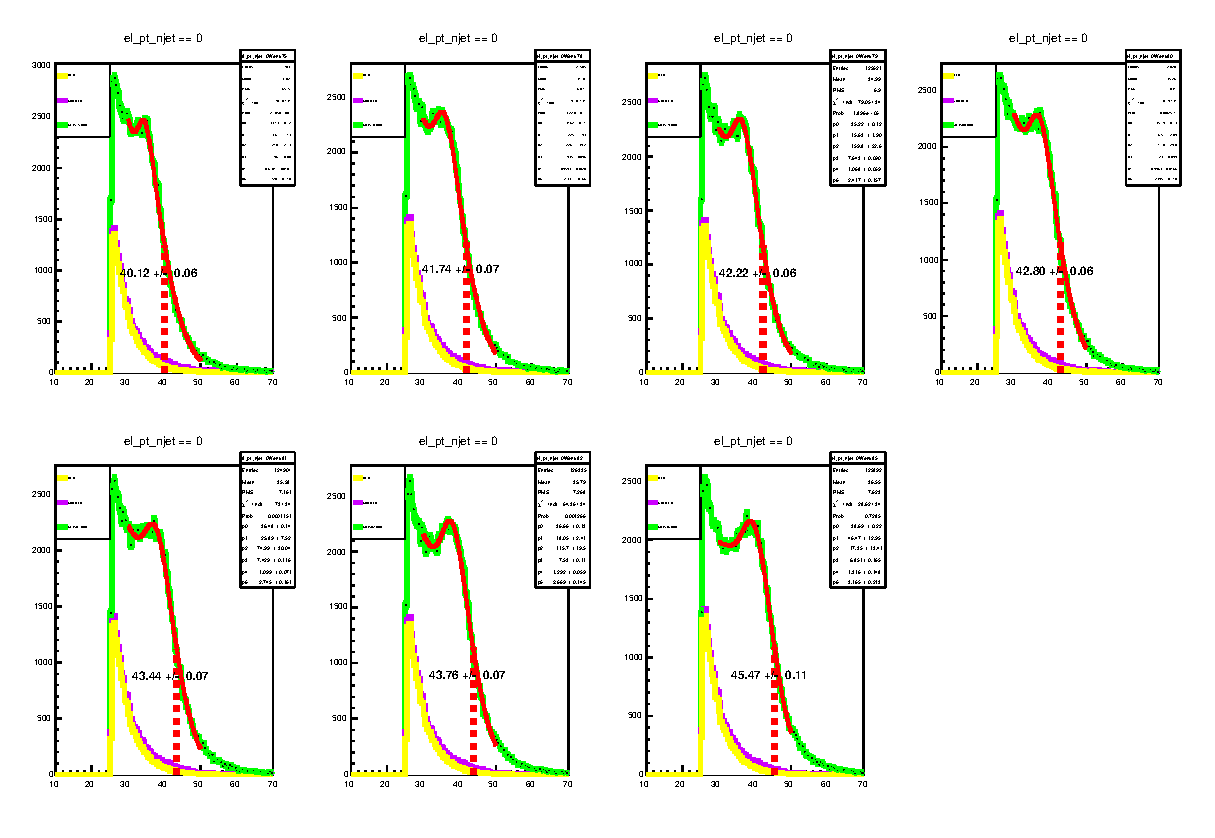
\includegraphics[width=\textwidth]{data/img/gauge_037.eps}
\caption{Gauge measurements for QCD scale factor 0.37 and fit range 30 - 50 GeV}
\end{figure}

\begin{figure}
\centering
\includegraphics[width=\textwidth]{data/img/gauge_033_i_30_60.eps}
\caption{Gauge measurements for QCD scale factor 0.33 and fit range 30 - 60 GeV}
\end{figure}
\begin{figure}
\centering
\includegraphics[width=\textwidth]{data/img/gauge_033_i_30_70.eps}
\caption{Gauge measurements for QCD scale factor 0.33 and fit range 30 - 70 GeV}
\end{figure}
\begin{figure}
\centering
\includegraphics[width=\textwidth]{data/img/gauge_033_i_35_55.eps}
\caption{Gauge measurements for QCD scale factor 0.33 and fit range 35 - 55 GeV}
\end{figure}

\subsection{Wenu dataset fits}
\begin{figure}
\centering
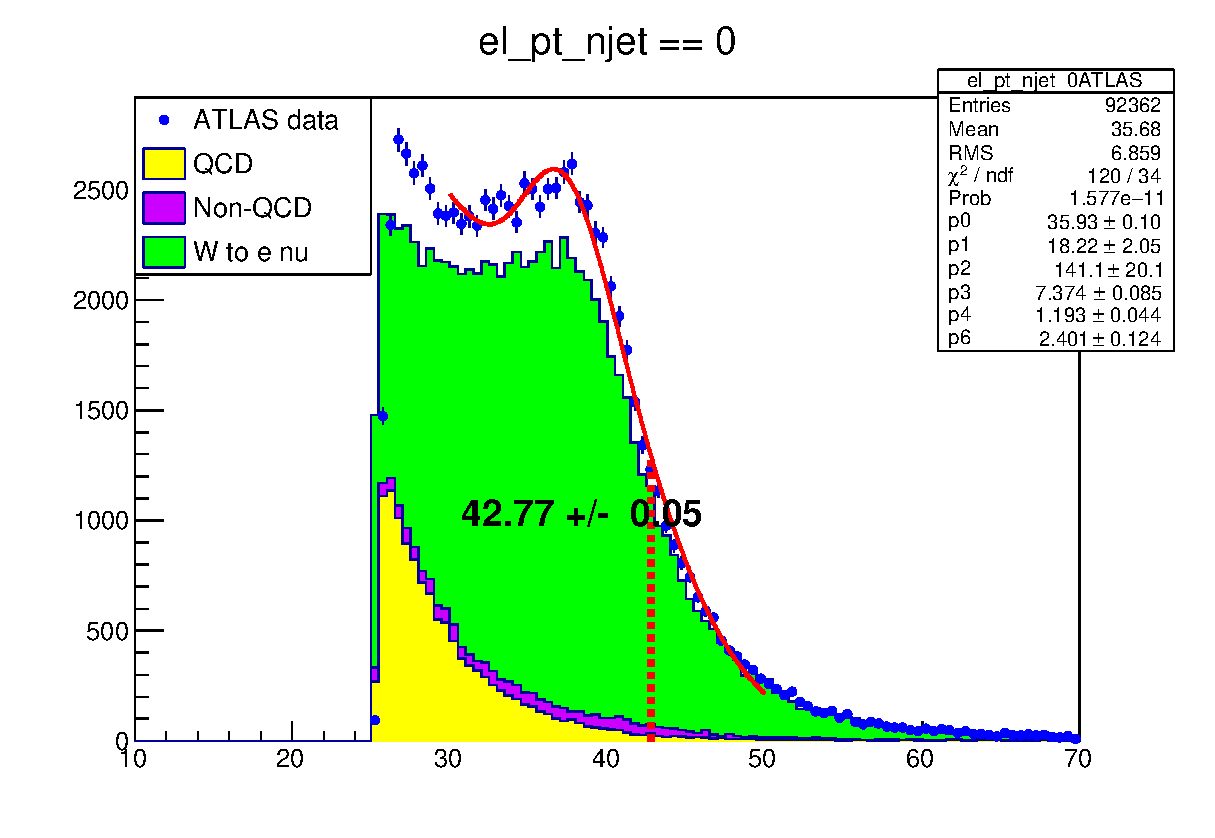
\includegraphics[width=\textwidth]{data/img/halfmax_Wenu_031.eps}
\caption{Fit to Wenu data for QCD scale factor 0.31 and fit range 30 - 50 GeV}
\end{figure}
\begin{figure}
\centering
\includegraphics[width=\textwidth]{data/img/halfmax_Wenu_033.eps}
\caption{Fit to Wenu data for QCD scale factor 0.33 and fit range 30 - 50 GeV}
\end{figure}
\begin{figure}
\centering
\includegraphics[width=\textwidth]{data/img/halfmax_Wenu_035.eps}
\caption{Fit to Wenu data for QCD scale factor 0.35 and fit range 30 - 50 GeV}
\end{figure}
\begin{figure}
\centering
\includegraphics[width=\textwidth]{data/img/halfmax_Wenu_037.eps}
\caption{Fit to Wenu data for QCD scale factor 0.37 and fit range 30 - 50 GeV}
\end{figure}

\begin{figure}
\centering
\includegraphics[width=\textwidth]{data/img/halfmax_Wenu_033_i_30_60.eps}
\caption{Fit to Wenu data for QCD scale factor 0.33 and fit range 30 - 60 GeV}
\end{figure}
\begin{figure}
\centering
\includegraphics[width=\textwidth]{data/img/halfmax_Wenu_033_i_30_70.eps}
\caption{Fit to Wenu data for QCD scale factor 0.33 and fit range 30 - 70 GeV}
\end{figure}
\begin{figure}
\centering
\includegraphics[width=\textwidth]{data/img/halfmax_Wenu_033_i_35_55.eps}
\caption{Fit to Wenu data for QCD scale factor 0.33 and fit range 35 - 55 GeV}
\end{figure}

\subsection{Zee dataset fit}
\begin{figure}
\centering
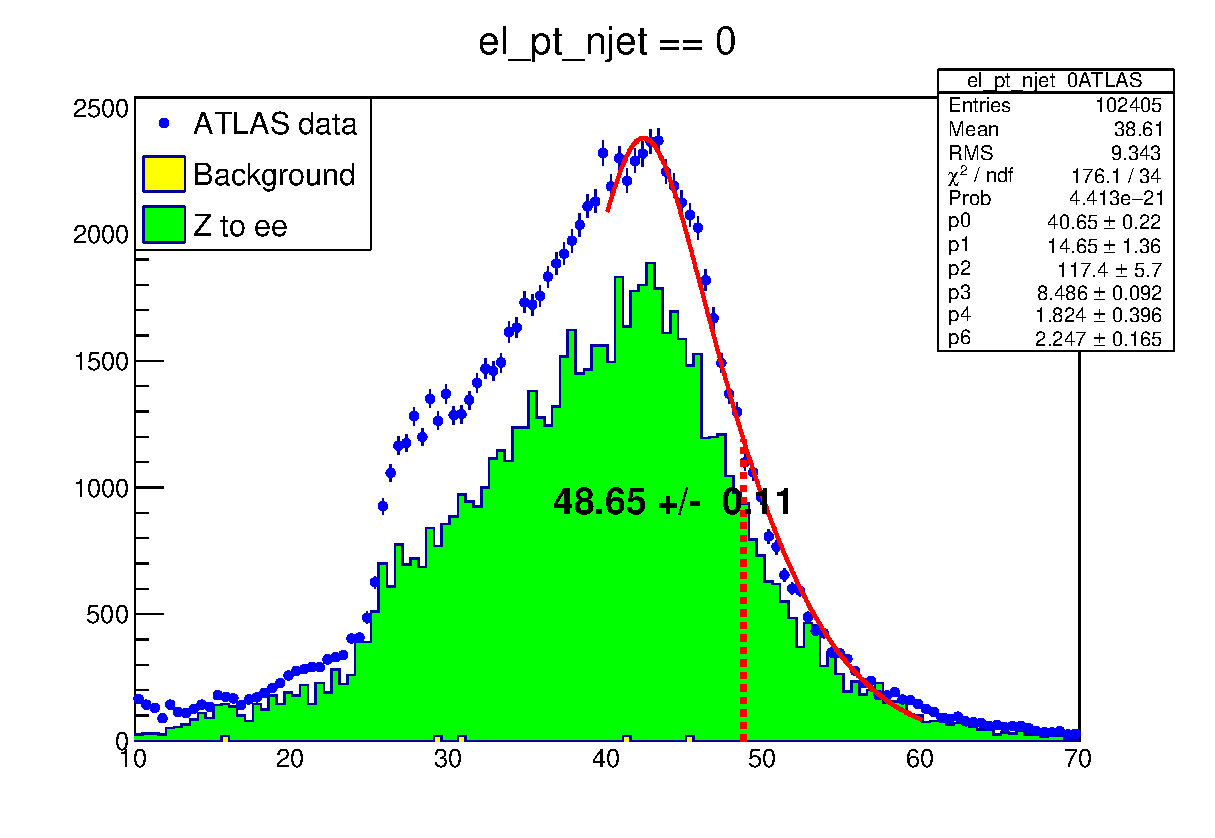
\includegraphics[width=\textwidth]{data/img/halfmax_Zee_033.eps}
\caption{Fit to Zee data for QCD scale factor 0.33 and fit range 30 - 50 GeV}
\end{figure}

\end{document}
